
\begin{figure}[t!]
\begin{center}
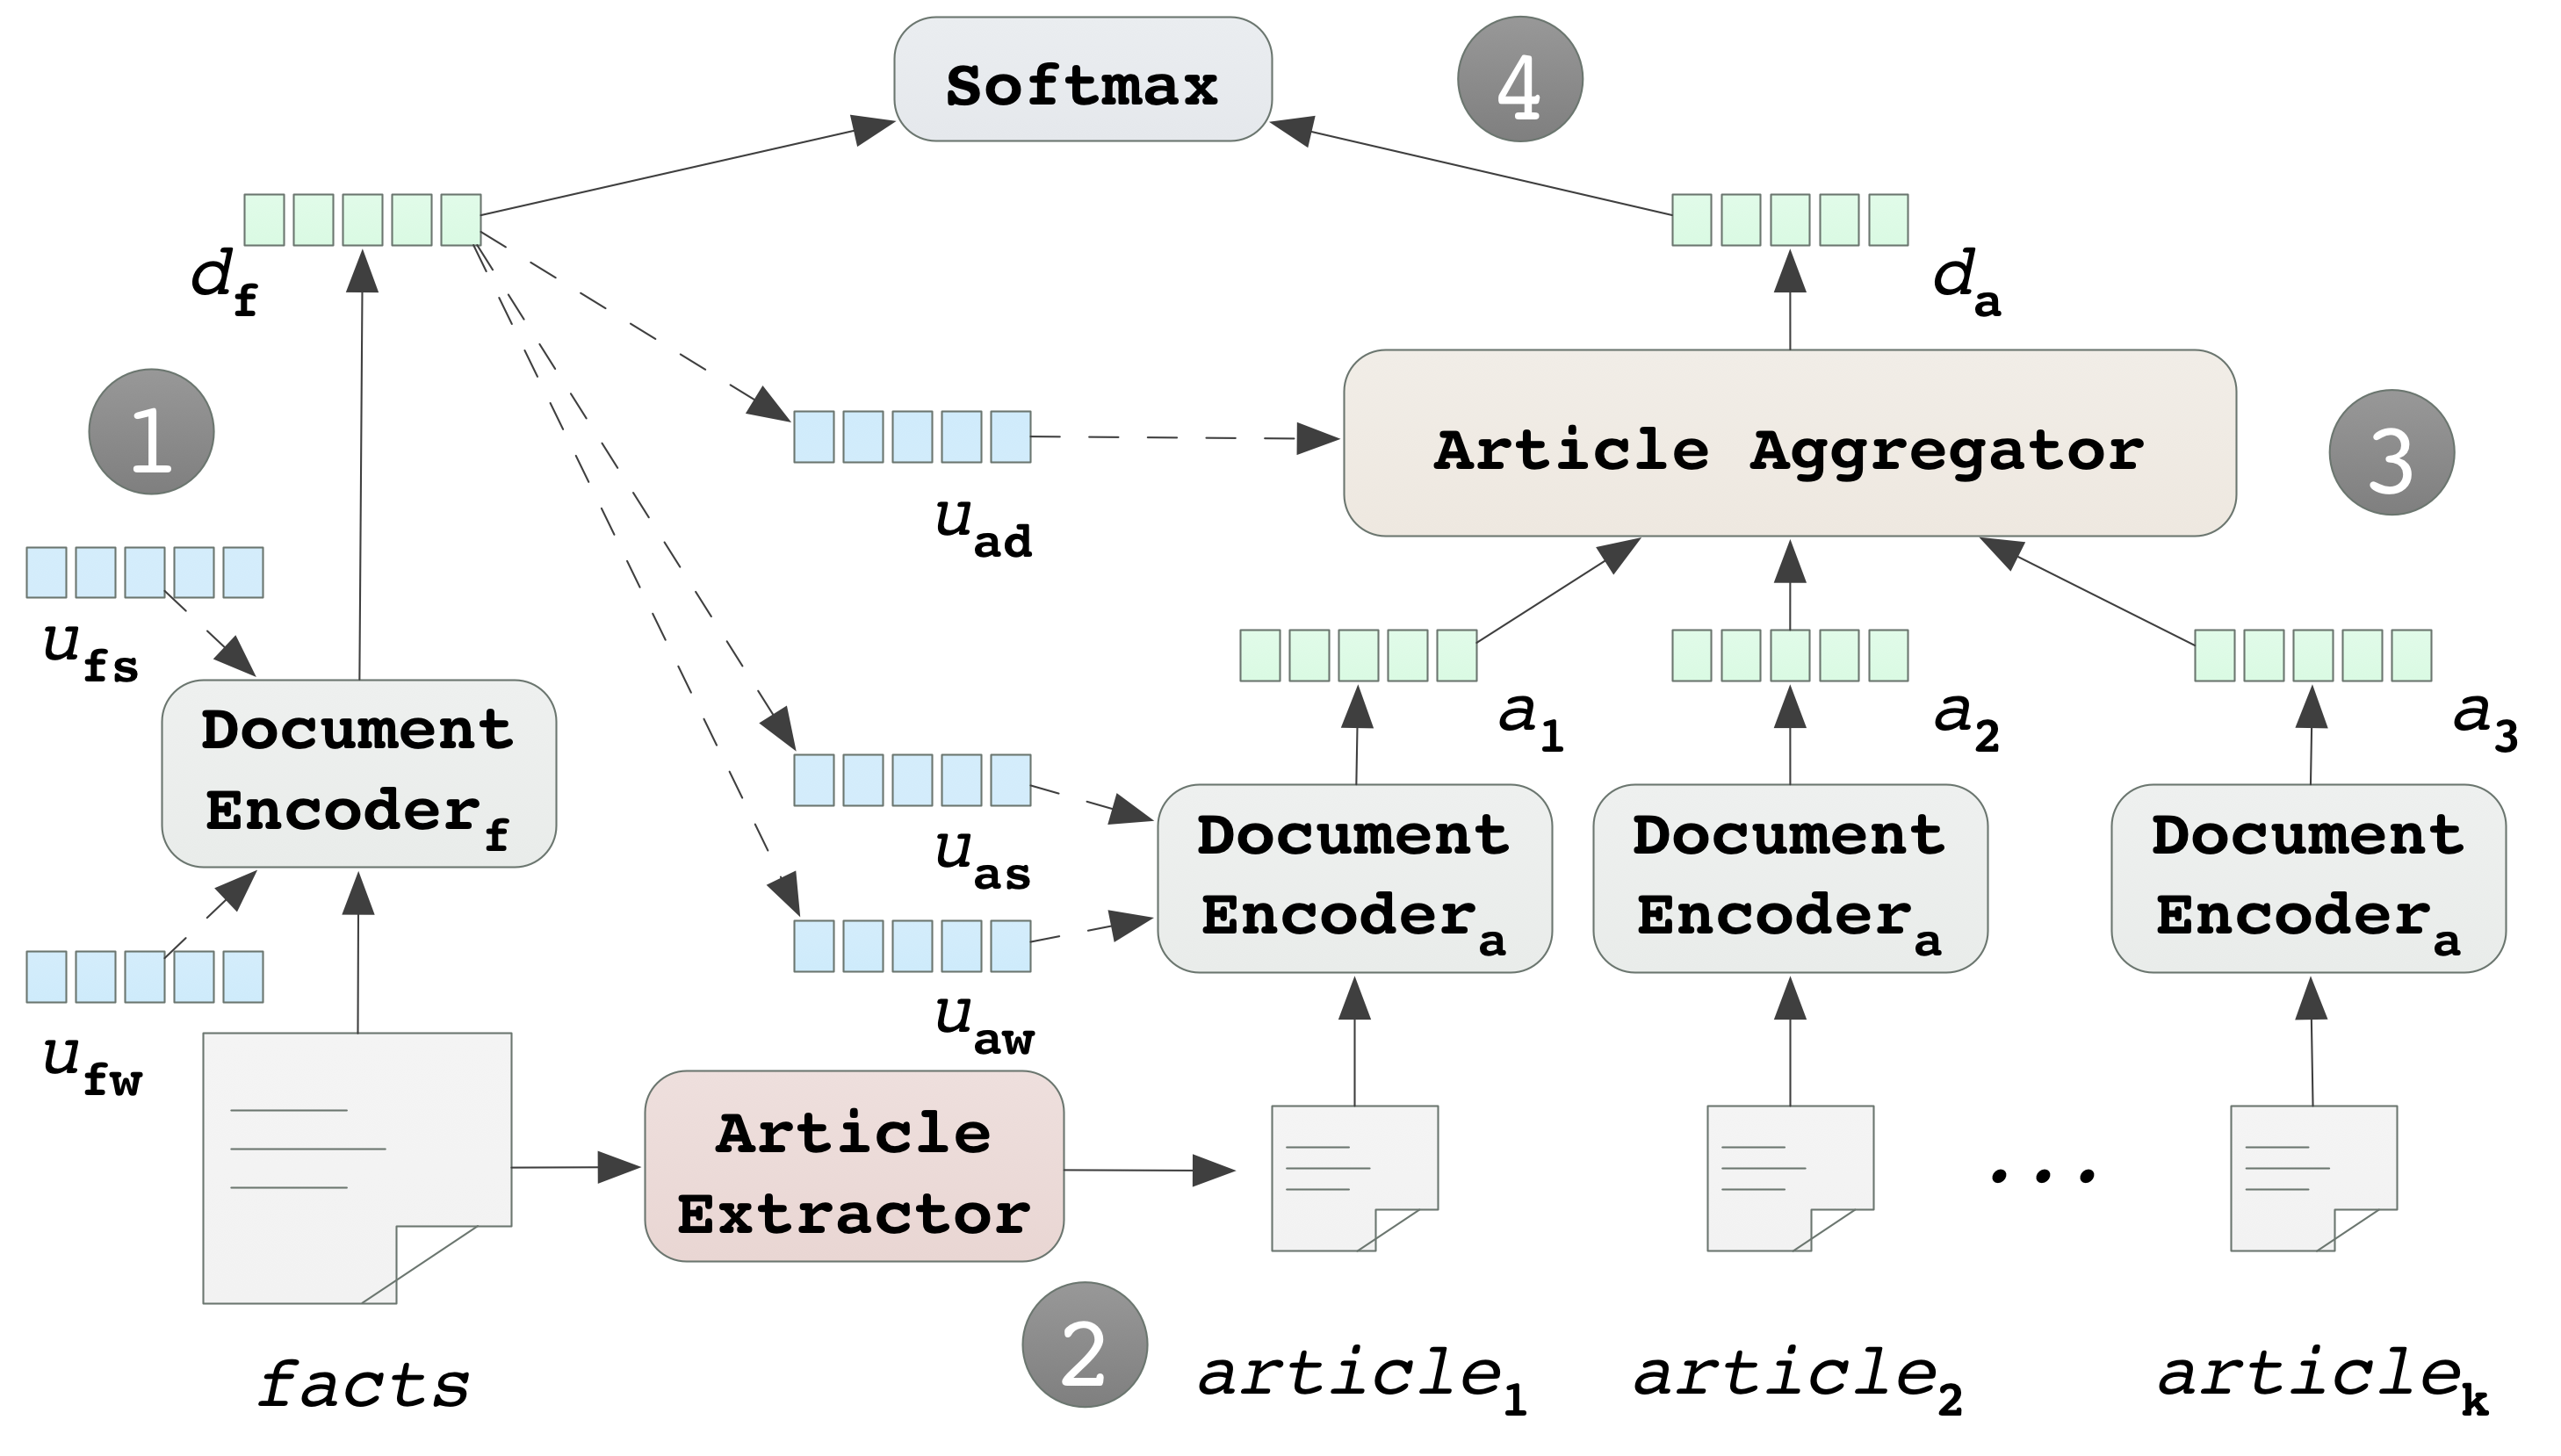
\includegraphics[width=0.48\textwidth]{figures/charge_pred_overview.png}	
\caption{Overview of Our Model}
\label{fig_model_framework}
\end{center}
\end{figure}

\section{Our Approach}
In order to generate reasonable charge prediction, our approach follows four steps as depicted in Figure \ref{fig_model_framework}. 
(1) The input fact description is fed to a document encoder to generate the fact embedding $\mathbf{d_f}$.
(2) Concurrently, the input fact description is also passed to a relevant article extractor to find top $k$ relevant law articles. 
(3) Each article is fed to another document encoder, and the article embeddings are further passed to an article aggregator to produce the aggregated article embedding $\mathbf{d_a}$. Meanwhile, three global attention vectors, i.e., $\mathbf{u_{aw}}$, $\mathbf{u_{as}}$ and $\mathbf{u_{ad}}$, are generated from the fact embedding $\mathbf{d_f}$ for the document encoder and the article aggregator. 
(4) Finally, $\mathbf{d_f}$ and $\mathbf{d_a}$ are concatenated and passed to a softmax classifier to predict the charge distribution of the input case.
\orange{what is the best way to organize this section?}

%The fact-based charge classification task can be formatted as a multi-label document classification task. The input is several sentences describing the facts of a case, and the output is multiple charges related to the case. Since usually multiple elements are required to constitute a charge (for example, the charge of acceptance of bribes requires the defendant to illegally accepts another person's money, and the defendant should also be a state functionary), the recurrent neural network (RNN) seems like a natural fit for the task. Considering the fact that only a small portion of the facts are crucial for the determination of charges, we also use attention mechanism in our model. Since the HAN model  satisfies many of our requirements except the multi-label classification capability, we use the framework of the HAN model for document embedding, but replace the output module and the loss function with ones that are compatible with the multi-label classification task. Furthermore, to take the information of article into account, we add another article attention module to incorporate the information of relevant articles to the model.

\subsection{Document Encoder}
% Our document encoder module is based on the framework of Hierarchical Neural Network (HAN) proposed by \cite{yang2016hierarchical}. The overview of our document encoder is shown in Figure \ref{fig_doc_encoder}. 
Intuitively, a sentence is a sequence of words and a document is a sequence of sentences. As suggested by previous works \cite{tang2015document,yang2016hierarchical}, the document embedding problem can be converted to two sequence embedding problems, i.e., embedding sequence of words and embedding sequence of sentences (see Figure \ref{fig_doc_encoder}). Therefore, the key problem of document embedding lies in building an effective sequence encoder. \todo{describe Figure \ref{fig_doc_encoder} somewhere}

\begin{figure}[htbp]
\begin{center}
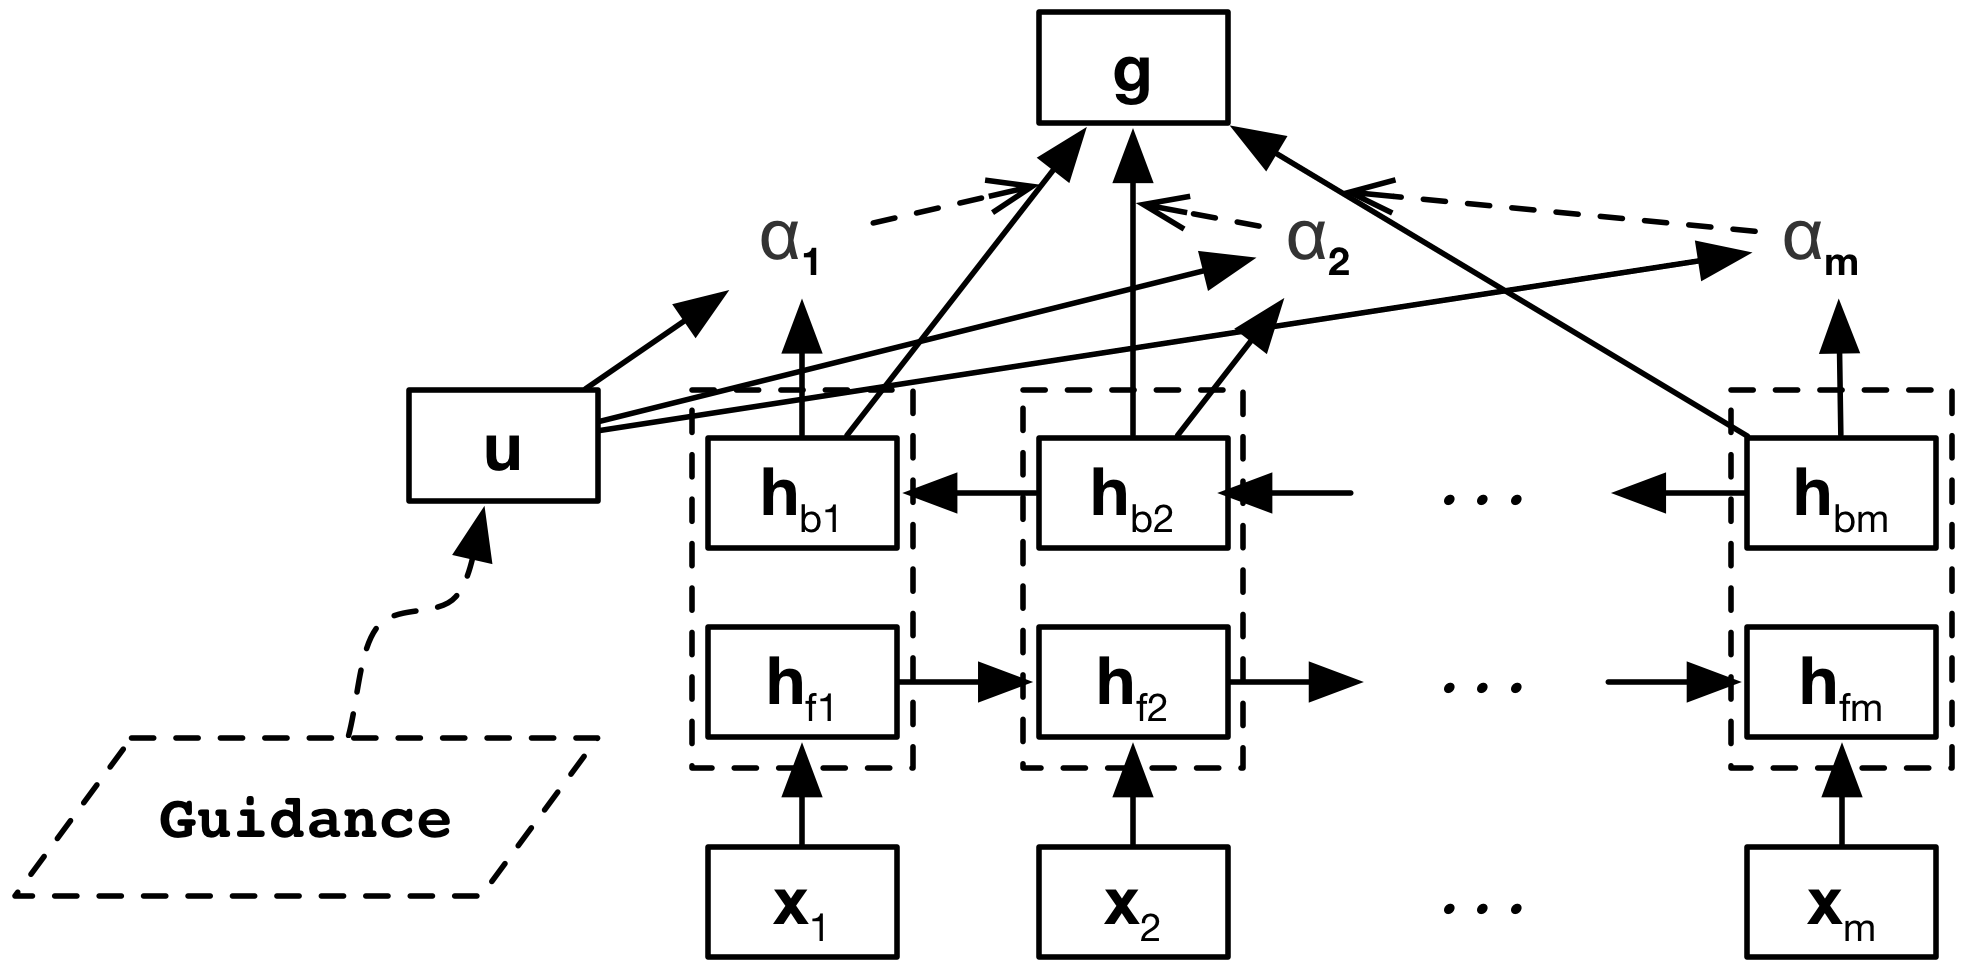
\includegraphics[width=0.45\textwidth]{figures/attentive_seq_encoder.png}	
\caption{Attentive Sequence Encoder}
\label{fig_seq_encoder}
\end{center}
\end{figure}

\begin{figure}[htbp]
\begin{center}
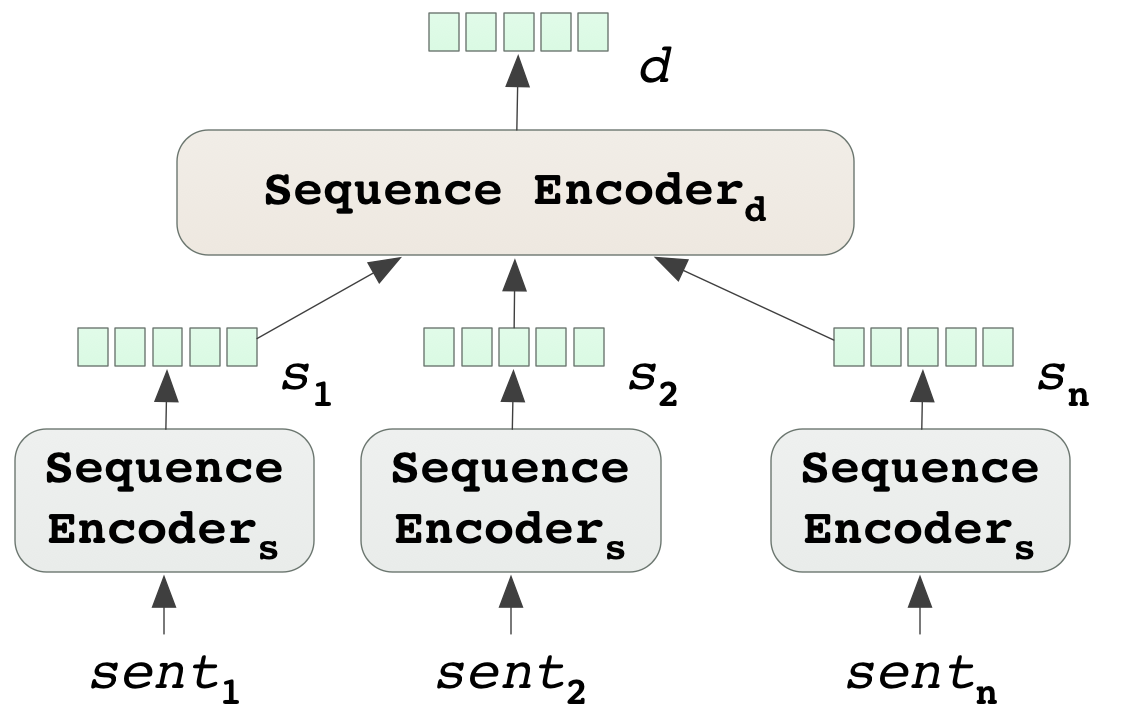
\includegraphics[width=0.35\textwidth]{figures/document_encoder.png}	
\caption{Document Encoder}
\label{fig_doc_encoder}
\end{center}
\end{figure}

\paragraph{Bi-GRU Sequence Encoder} 


It is important to consider the correlation of the elements when encoding a sequence. Here we use the bi-directional GRU model  for sequence encoding, which is an extension of the GRU model \cite{cho2014learning} that use a forward and a backward GRU to model the sequence separately, and then combine the results of both GRUs. Given a sequence $[x_1, x_2, ..., x_T]$ where $x_t$ is the embedding of the element at position $t$, the encoding result is:

\begin{equation}
%\overrightarrow{h}_t = \overrightarrow{GRU}(x_t)
h_{ft} = GRU_f(x_{t})
\end{equation}
\begin{equation}
%\overleftarrow{h}_t = \overleftarrow{GRU}(x_t)
h_{bt} = GRU_b(x_{t})
\end{equation}
\begin{equation}
%h_t = [\overrightarrow{h}_t , \overleftarrow{h}_t]
h_t = [h_{ft}, h_{bt}]
\end{equation}
where $GRU_f$ is the forward GRU that processes the sequence from left to right, and $GRU_b$ is the backward GRU that processes the sequence from right to left. $h_t$ is the state of the bi-directional GRU model at time $t$, which is generated by concatenating the states of the two GRU models at time $t$. The state of a single GRU model at time $t$ is calculated by: 
\begin{equation}
h_t=(1-z_t)\odot h_{t-1} + z_t\odot \tilde{h}_{t}
\end{equation}
with a little abuse of annotations, $h_t$ here stands for the state of time $t$ of a single GRU model. $z_t\in{[0,1]}$ is the update gate, $h_{t-1}$ is the previous state, $\tilde{h}_{t}$ is the candidate state and $\odot$ is element wise product. The update gate that controls the interpolation of the previous state and the candidate state is calculated by:
 \begin{equation}
z_t=\sigma(W_z x_t+U_z h_{t-1} + b_z)
\end{equation}
where $x_t$ is the input at time $t$, $W_z$ and $U_z$ are weight matrices, $b_z$ is the bias and $\sigma$ is the sigmoid function. The candidate state $\tilde{h}_{t}$ is calculated by:
\begin{equation}
\tilde{h}_{t}=tanh(W_h x_t + r_t\odot U_h h_{t-1} + b_h)
\end{equation}
where $r_t$ is the reset gate, which is controls how information does the previous state contributes to the candidate state, and it is calculated by:
\begin{equation}
r_t=\sigma(W_r x_t + U_r h_{t-1} + b_r)
\end{equation}



\paragraph{Element Attention}
Since not all elements of a sequence contributes equally to the final output, the attention mechanism is used to select the most import parts of a sequence. Given the GRU output $[h_1, h_2, ..., h_T]$ of a sequence, we calculate a sequence of attention values $[\alpha_1, \alpha_2, ..., \alpha_T]$ where $\alpha_t \in [0, 1]$ and $\sum_t{\alpha_t}=1$. The final embedding of the sequence is calculated as:
\begin{equation}
h = \sum_{t=1}^{T}{\alpha_t h_t}
\label{seq_embed}
\end{equation}
where the attention value $\alpha_t$ is calculated by:
\begin{equation}
v_t = tanh(Wh_t)
\label{eq_att_transform}
\end{equation}
\begin{equation}
\alpha_t=\frac{exp(v_t^T u)}{\sum_t{exp(v_t^T u)}}
\label{gen_att}
\end{equation}
where $W$ is a weight matrix, and $u$ is global attention vector that is used to distinguish import elements from unimportant ones. 

\paragraph{Putting Everything Together}
As shown in Figure \ref{doc_embed}, we first use the bi-directional GRU and a word-level attention vector $u_w$ to get the sentence embedding $s_i$. Then another bi-directional GRU and a sentence-level attention vector $u_s$ is applied to the sentence sequence $[s_1, s_2, ..., s_n]$ to get the document embedding $d$.

\subsection{Generating Output}
There are two commonly used methods for multi-label classification in neural network models. The first one is to consider the multi-label classification problem with $L$ labels as $L$ binary classification problem. It uses sigmoid function in the output layer and binary cross entropy as loss function. This method performs well in many multi-label text classification problems \cite{nam2014large}.

The second method uses the softmax function to generate outputs. It first convert the multi-label target to a probability distribution. For example, suppose there are 4 classes and one datum belongs to class 0 and class 2. This method will convert the $y=[1, 0, 1, 0]$ to $y=[0.5, 0, 0.5, 0]$, and cross entropy will be used as the loss function. After training, a threshold $\tau$ is selected and all the classes that have a score higher than $\tau$ will be considered as positive classes. This method proves to work well in the natural language query classification task \cite{kurata2016improved}. 

In our pilot experiments, we find that the first method converges about 5 times slower than the second method in our dataset, and the second method also produces better results. We think this phenomenon happens because only a small fraction of our data are multi-label data. Therefore the second method, which uses the same output function as multi-class classification tasks, works better in our task. In this paper, we will use the second method.

Specifically, if only fact description is used, the fact embedding $d$ is first passed to a multi-layer perceptron (MLP). The MLP output $d'$ is further fed to a softmax function to generate the class distribution $o$. The cross entropy loss function is:
\begin{equation}
\label{original_loss}
Loss_d= -\sum_{i=1}^N\sum_{l=1}^L{y_{il} log(o_{il})}
\end{equation} 
where $N$ is the number of training data, $L$ is the number of charges, $y_{il}$ and $o_{il}$ are the target and predicted probability of the $l^{th}$ charge of the $i^{th}$ datum. 

If both fact description and relevant law articles are used, the MLP input is the concatenation of of the fact embedding $d$ and the aggregated article embedding $d_a$ (see Section \ref{Embed Relevant Articles}).

\subsection{Extracting Relevant Articles}
\label{Extracting Relevant Articles}
We consider the relevant article extraction task as a multi-label classification task. In our dataset, there are 321 law articles and we consider this task as 321 binary classification problems. 
In this task, we use bag-of-words TF-IDF features. First, chi-square method is applied to the original feature set for feature selection. Then SVM with linear kernel is used for the binary classification. Finally, the articles are ranked by the score output by SVM and the top $k$ articles are kept for each judgement document.

\subsection{Embed Relevant Articles}
\label{Embed Relevant Articles}
As shown in Figure \ref{fig_model_framework}, each article is first passed to the document embedding module to generate the article embedding $a_j, j\in [1, k]$. Different from the fact embedding module, the word level attention vector $u_{aw}$ and sentence level attention vector $u_{as}$ here are generated by linear transformations of the fact embedding $d$ rather than randomly initialization:
\begin{equation}
u_{aw} = W_w d + b_w
\end{equation}
\begin{equation}
u_{as} = W_s d + b_s
\end{equation}

To model the phenomenon that some articles tend to co-exist while others may be exclusive to each other, we also consider the $k$ articles as a sequence, and the bi-GRU model is used to embed the context of each article. Similarly, we also generate an article level attention vector $u_{a}$ by:
\begin{equation}
u_a = W_a d + b_a
\end{equation}
and $u_a$ is further used to generate article attention using Equation \ref{eq_att_transform} and \ref{gen_att}. After that, Equation \ref{seq_embed} is used to generate the aggregated article embedding $d_a$. 

\subsection{Guided Article Attention}
Note that each judgement document also contains gold standard relevant law articles that can be applied to this case. Therefore, we can use this information to guide the article attention module. Specifically, given the $k$ articles returned by the relevant article extraction module, we want the article attention distribution $\alpha=[\alpha_1, \alpha_2, ..., \alpha_k]$ to simulate the target distribution $t\in\mathbb{R}^k$:
\begin{equation}
t_j=
\begin{cases}
1/|\mathbb{A}|,	& j\in \mathbb{A}\\
0,	& else
\end{cases}
\end{equation}
where $\mathbb{A}$ is the set of indices of the articles in the top $k$ extracted articles that belongs to gold standard articles, and $|\mathbb{A}|$ is the size of set $\mathbb{A}$. 

Therefore, the final loss function is:
\begin{equation}
\label{final_loss}
Loss = -\sum_{i=1}^N(\sum_{l=1}^L{y_{il} log(o_{il})} + \beta \sum_{j=1}^k{t_{ij} log(\alpha_{ij})})
\end{equation}
where the left side is the cross entropy between the target charge distribution and the predicted charge distribution defined in Equation \ref{original_loss}, and the right side is the cross entropy between the target article distribution and the article attention distribution. 